%-----------------------------------------------------------------------------%
\chapter{\babSatu}
%-----------------------------------------------------------------------------%

This chapter explains the background of this research and the problem to be
solved by this research.

%-----------------------------------------------------------------------------%
\section{Research Background}
%-----------------------------------------------------------------------------%

When the web platform was in its early stages, every part of a web application
was programmed without the help of a web framework. At that time, developing a
web application required extensive knowledge of how the web works. Depending on
the web application, the programmers might need deep understanding of the
Hypertext Transfer Protocol (HTTP), the Hypertext Markup Language (HTML), and
other things such as databases. If the web application was not programmed
correctly, it could lead to a lot of errors and security holes in the web
application.

Web frameworks aim to solve this problem by providing a standard way to build
web applications. Web frameworks help eliminate the overhead of implementing
common parts of web applications such as the HTTP layer, the user interface
layer, and the database layer. By using a web framework, programmers can build
web applications more quickly and safely by focusing more on the business logic
of the web application itself instead of the more intricate details.

Among the widely-used web frameworks is Django, a free and open-source web
framework written in Python.\footnote{\url{https://djangoproject.com}} Django
encourages rapid development and clean, pragmatic design \cite{django}. Django
was designed to help developers build their website quickly and securely with
scalability in mind.

One of the main features of Django is an object-relational mapping (ORM) tool
in the database layer \cite{django}. Django's ORM tool provides an
object-oriented abstraction of the database by mapping data models (represented
as Python classes) to tables in a relational database. The columns of a
database table are defined as attributes (called fields) inside the model
class. Using Django's ORM tool, programmers can interact with the database by
writing Python code instead of writing Structured Query Language (SQL)
statements. The abstraction provided by Django's ORM tool also helps
programmers avoid common mistakes that can lead to security issues such as SQL
injections.

Relational database systems can be used to manage structured data in the form
of tables with strict standards. The tables in a relational database can be
linked (related) based on data that is common to each table. Relating the
tables is possible because relational database systems enforce the data to be
consistent with a defined schema. This consistency is implemented according to
the Atomicity, Consistency, Isolation, and Durability (ACID) properties of
relational database transactions \cite{abramova_nosql}. These properties
guarantee that the data is valid despite any events of power failures, errors,
and other accidents.

Meanwhile, there has been an increase in the popularity of non-relational
databases, commonly known as NoSQL databases \cite{paul_nosql}. NoSQL
encourages the simplicity of database design, which makes the process of
scaling the database to multiple clusters of machines easier
\cite{leavitt_nosql}. Instead of tables, most NoSQL databases store data in the
form of key-value stores, document stores, or graphs \cite{strauch_nosql}.
NoSQL databases are also considered as more flexible due to its dynamic schema.
For example, some document-based NoSQL databases store data in JavaScript
Object Notation (JSON) format, which means that the schema is defined in the
data itself.

However, NoSQL databases also have their own downsides. Most NoSQL databases do
not fully support the ACID principles found in relational databases
\cite{cattell_nosql}. Instead of the ACID principles, they focus on the
Basically Available, Soft state, and Eventually consistent (BASE) principles
\cite{abramova_nosql}. The BASE principles state that the data should be
available most of the time (it can support partial failures), the data does not
have to be consistent at all times (soft state), but the data is guaranteed to
be consistent at some point (eventually). In addition, they also lack the
ability to perform joins across tables due to their horizontal data
distribution \cite{pokorny_nosql} and their use of denormalized data, which
makes it harder to work with entity relations.

To compete with NoSQL databases, some relational database systems have come up
with their own ways to provide more flexibility for the data model. Some of
them provide the option to combine structured data with some form of
semi-structured data, most commonly in JSON format \cite{mariadb_json}. On
these databases, the user can store JSON data in a table column. The
possibility to store JSON data in a relational database gives all the benefits
of using a relational database, while still allowing the simplicity and
flexibility of semi-structured data.

From version 1.9 until version 3.0, Django had provided an implementation of
\verb|JSONField|. However, it was exclusively available for PostgreSQL. This
\verb|JSONField| allowed its users to store and query JSON data in a relational
database column using the \verb|jsonb| data type found only on PostgreSQL at
the time.\footnote{PostgreSQL has two JSON data types: \code{json} and
\code{jsonb}. Django's \code{JSONField} uses \code{jsonb}.} Django officially
supports PostgreSQL, MariaDB, MySQL, SQLite, and Oracle Database backends. Over
the years since the initial PostgreSQL \verb|JSONField| implementation, those
database systems have developed their own support for managing JSON data.
However, Django had yet to implement \verb|JSONField| for database backends
other than PostgreSQL.

The limited support for \verb|JSONField| prompted the Django community to
create their own \verb|JSONField| implementations for other database backends.
Some of them target one specific database backend and utilize various functions
provided by the database system to add extended querying capabilities
\cite{mysql_jsonfield, oracle_jsonfield}. Some other implementations
focus on cross-database support, thus they are only implemented as text-based
fields that do not have any extended querying capabilities
\cite{ryan_jsonfield}.

The individual efforts for implementing \verb|JSONField| result in the
abundance of third-party \verb|JSONField| packages on PyPI.\footnote{The Python
Package Index (PyPI) is a software repository for the Python programming
language (\mbox{\url{https://pypi.org}}).} Some of them are very popular, such as the
\mbox{jsonfield} package that has more than 1100 stars on GitHub
\cite{ryan_jsonfield}. While this indicates a popular demand for
\verb|JSONField|, it also indicates a fragmentation problem in the Django
ecosystem as people use different \verb|JSONField| packages. Thus, there is a
motivation to bring \verb|JSONField| into Django's core model fields.

There is also a motivation to implement additional validations for JSON data in
a \verb|JSONField|. By default, the validation for JSON data on the database
level only validates the syntax and not the information contained in the data
iself. Meanwhile, the flexibility of JSON data in a \verb|JSONField| might
introduce invalid information or abnormalities within the data. For example,
the data might refer to a nonexisting record in one of the database tables. To
ensure the correctness of the JSON data in a \verb|JSONField|, additional
validations need to be implemented.

With the motivations described in the previous paragraphs, this research aimed
to implement \verb|JSONField| in Django and demonstrate validation examples for
\verb|JSONField|. The new implementation of \verb|JSONField| would have
cross-database support, extended querying support, and compatibility with the
previous \verb|JSONField| implementation. Additional validations for
\verb|JSONField| would be demonstrated by creating a Django project that would
utilize Django's validation features. If these targets were achieved, they
would hopefully benefit the Django community by bringing \verb|JSONField| into
the core model fields in Django and giving validation examples for
\verb|JSONField|.

%-----------------------------------------------------------------------------%
\section{Research Questions}
%-----------------------------------------------------------------------------%

Based on the aforementioned research background, the following questions are
constructed for this research:

\begin{enumerate}
    \item How can \verb|JSONField| in Django be reimplemented with multiple
          databases support and compatibility with the PostgreSQL-only
          \verb|JSONField| implementation?
    \item How can Django users enforce validation rules on a \verb|JSONField|?
\end{enumerate}

%-----------------------------------------------------------------------------%
\section{Research Objectives}
%-----------------------------------------------------------------------------%

The objectives of this research are to:

\begin{itemize}
    \item Implement a new \verb|JSONField| that can be used on all database
          backends supported by Django without breaking compatibility with the
          PostgreSQL-only \verb|JSONField|.
    \item Demonstrate how semi-structured data in a \verb|JSONField| can be
          validated.
\end{itemize}

%-----------------------------------------------------------------------------%
\section{Research Benefits}
%-----------------------------------------------------------------------------%

This research would hopefully bring the following benefits:

\begin{itemize}
    \item Provide Django users with a \verb|JSONField| that has a mostly
          consistent experience on all database backends supported by Django.
    \item Give insights to Django users about the inner workings of
          \verb|JSONField| and validation examples of \verb|JSONField|.
\end{itemize}

%-----------------------------------------------------------------------------%
\section{Research Scope}
%-----------------------------------------------------------------------------%

The following assumptions were made prior to the execution of this research:

\begin{itemize}
    \item The \verb|JSONField| implementation would be submitted as a pull
          request and merged to the upstream Django repository instead of being
          made as a separate package.
    \item The \verb|JSONField| implementation would have to take into account
          the limitations of each database backend, thus there might be
          features that behave differently or would not be supported on some
          database backends.
\end{itemize}

%-----------------------------------------------------------------------------%
\section{Research Position}
%-----------------------------------------------------------------------------%

\begin{figure}
	\centering
    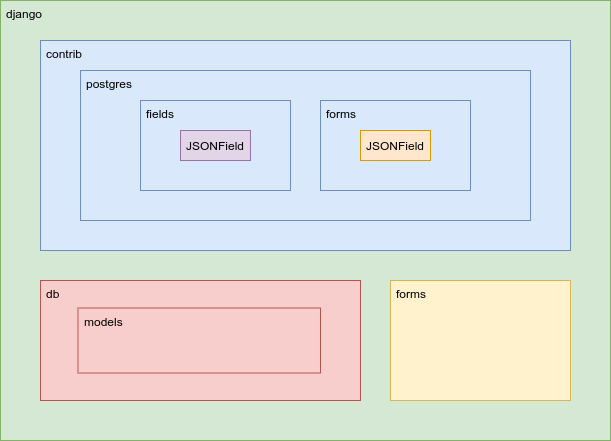
\includegraphics[width=0.85\textwidth]{pics/position1.png}
	\caption{\code{JSONField} classes in Django prior to this research.}
	\label{fig:position1}
\end{figure}

Before this research, the existing \verb|JSONField| implementation was included
in the \verb|django.contrib.postgres.fields| and
\verb|django.contrib.postgres.forms| modules \cite{django30_modeljsonfield,
django30_formjsonfield}. The \verb|django.contrib.postgres| module contains
model fields, form fields, and other features that only work with the
PostgreSQL database backend. The locations of the \verb|JSONField| classes in
Django prior to this research are illustrated by \autoref{fig:position1} (note
that other Django modules are omitted for brevity).

\begin{figure}
	\centering
    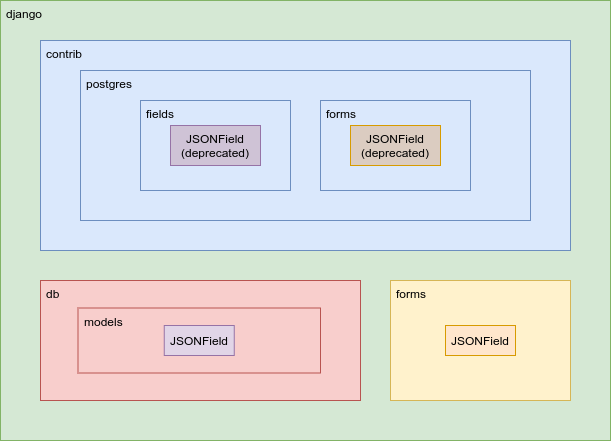
\includegraphics[width=0.85\textwidth]{pics/position2.png}
	\caption{\code{JSONField} classes in Django after this research.}
	\label{fig:position2}
\end{figure}

This research brought \verb|JSONField| and other related classes to the
\verb|django.db.models| module for the model field and to the
\verb|django.forms| module for the form field. Consequently, the previous
implementation was deprecated as of the Django 3.1 release. The previous
implementation would also be removed in the next major release, Django 4.0.

\begin{figure}
	\centering
    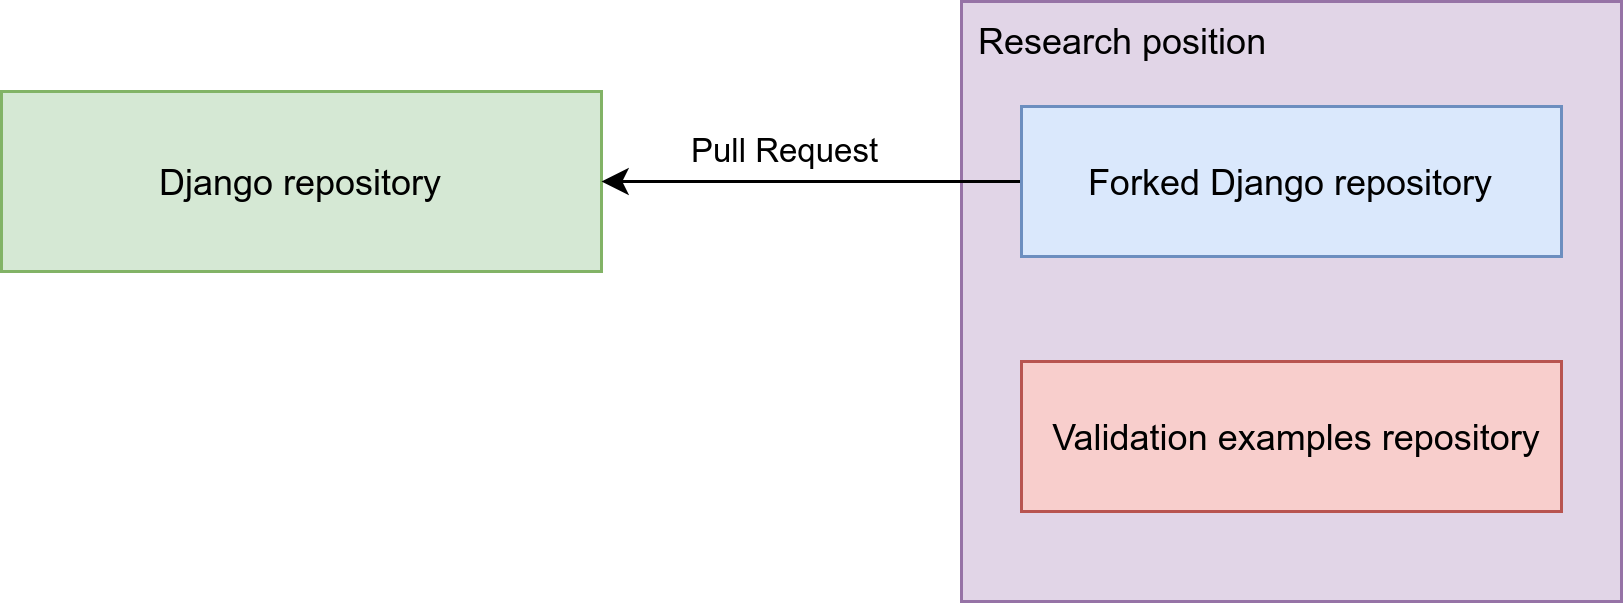
\includegraphics[width=0.85\textwidth]{pics/position3.png}
	\caption{The position of this research.}
	\label{fig:position3}
\end{figure}

This research is mainly split into two parts: the \verb|JSONField|
implementation and the validation examples. The \verb|JSONField| implementation
part of the research was done on a Git branch in a GitHub fork of the Django
repository.\footnote{\url{https://github.com/laymonage/django/tree/ticket_12990}}
The branch was submitted as a pull
request\footnote{\url{https://github.com/django/django/pull/12392}} to the
Django repository to fix ticket \#12990 on the Django issue tracker
\cite{ticket_12990} and was included in the Django 3.1.0 release. The pull
request allowed the Django contributors to review the code and give feedback on
the implementation. The data validation examples were created in a separate
repository in the form of a small Django project. The position of this research
is illustrated by \autoref{fig:position3}.

\begin{figure}
	\centering
    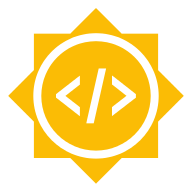
\includegraphics[width=0.25\textwidth]{pics/GSoC.png}
	\captionsource{The Google Summer of Code
        logo.}{\url{https://developers.google.com/open-source/gsoc/resources/marketing}}
	\label{fig:gsoc}
\end{figure}

The \verb|JSONField| implementation was mostly done as part of the Google
Summer of Code 2019 program. Google Summer of Code (GSoC) is an annual program
held by Google that is focused on introducing students to open-source software
development. In GSoC, students work on a three-month programming project under
the guidance of mentors from an open-source organization. The students are
compensated with a stipend from Google for their work. In turn, the
organizations can identify and bring in new contributors who implement new
features and hopefully continue to contribute to the organizations' projects.
In this case, the organization was the Django Software
Foundation.\footnote{\url{https://www.djangoproject.com/foundation}}

%-----------------------------------------------------------------------------%
\section{Research Steps}
%-----------------------------------------------------------------------------%

The following steps were conducted for the research:

\begin{enumerate}
    \item Preliminary research \\
    This step focused on learning how the Django object-relational mapping
    (ORM) tool works and how JSON data is supported on the database systems
    supported by Django. During this step, the underlying concepts of this
    research were studied to gain some insights on how to accomplish the
    research objectives.

    \item Experiments \\
    In this step, experiments were done by trying out existing \verb|JSONField|
    implementations, which included the PostgreSQL implementation in Django and
    third-party packages on the Python Package Index (PyPI). Some experiments
    were also done by modifying a third-party package to work better on
    different database backends.

    \item Implementation \\
    This step focused on the implementation of the \verb|JSONField| model
    field, form field, lookups, and transforms. This step was initially done by
    copying the existing implementation from the \verb|django.contrib.postgres|
    module to the \verb|django.db.models| and \verb|django.forms| modules. The
    tests for the existing implementation were also gradually copied. From
    there, the work was to modify the \verb|JSONField| implementation so that
    all tests could pass on all available database backends. After the
    \verb|JSONField| implementation was finished, this step was continued by
    implementing the data validation examples.

    \item Results Analysis \\
    In this step, the primary work was to ensure that the behavior of the new
    implementation is mostly consistent on all database backends. Additional
    work was also done to ensure that the new implementation is compatible with
    the PostgreSQL-only implementation. At the end of this step, the classes in
    the PostgreSQL-only implementation were deprecated and replaced by replicas
    that raise system warnings to remind programmers to update their code.
\end{enumerate}

%-----------------------------------------------------------------------------%
\section{Report Structure}
%-----------------------------------------------------------------------------%

The structure of this report is as follows:

\begin{itemize}
    \item Chapter 1 \babSatu \\
        This chapter covers the background, problem definition, objectives,
        scope, position, and steps of this research.
    \item Chapter 2 \babDua \\
        This chapter covers the results of the preliminary study done prior to
        executing the research.
    \item Chapter 3 \babTiga \\
        This chapter covers the design and analysis to prepare for the
        implementation.
    \item Chapter 4 \babEmpat \\
        This chapter covers the implementation of \verb|JSONField| and its
        extended querying capabilities.
    \item Chapter 5 \babLima \\
        This chapter covers the demonstration of validation rules applied on
        a \verb|JSONField| to validate the JSON data inside the field.
    \item Chapter 6 \babEnam \\
        This chapter covers the tests for \verb|JSONField| and the deprecation
        of the previous PostgreSQL-only implementation.
    \item Chapter 7 \kesimpulan \\
        This chapter covers the conclusions of the research and some
        recommendations for future research.
\end{itemize}
